% REMEMBER: You must not plagiarise anything in your report. Be extremely careful.

\documentclass{l4proj}

    
%
% put any additional packages here
%

\begin{document}

%==============================================================================
%% METADATA
\title{Fruit Cocktail - Optimised Microservice Deployment in the Cloud}
\author{Krishang Patney}
\date{\today}

\maketitle

%==============================================================================
%% ABSTRACT
\begin{abstract}
    Every abstract follows a similar pattern. Motivate; set aims; describe work; explain results.
    \vskip 0.5em
    ``XYZ is bad. This project investigated ABC to determine if it was better. 
    ABC used XXX and YYY to implement ZZZ. This is particularly interesting as XXX and YYY have
    never been used together. It was found that  
    ABC was 20\% better than XYZ, though it caused rabies in half of subjects.''
\end{abstract}

%==============================================================================

% EDUCATION REUSE CONSENT FORM
% If you consent to your project being shown to future students for educational purposes
% then insert your name and the date below to  sign the education use form that appears in the front of the document. 
% You must explicitly give consent if you wish to do so.
% If you sign, your project may be included in the Hall of Fame if it scores particularly highly.
%
% Please note that you are under no obligation to sign 
% this declaration, but doing so would help future students.
%
%\def\consentname {My Name} % your full name
%\def\consentdate {20 March 2018} % the date you agree
%
\educationalconsent


%==============================================================================
\tableofcontents

%==============================================================================
%% Notes on formatting
%==============================================================================
% The first page, abstract and table of contents are numbered using Roman numerals and are not
% included in the page count. 
%
% From now on pages are numbered
% using Arabic numerals. Therefore, immediately after the first call to \chapter we need the call
% \pagenumbering{arabic} and this should be called once only in the document. 
%
% Do not alter the bibliography style.
%
% The first Chapter should then be on page 1. You are allowed 40 pages for a 40 credit project and 30 pages for a 
% 20 credit report. This includes everything numbered in Arabic numerals (excluding front matter) up
% to but excluding the appendices and bibliography.
%
% You must not alter text size (it is currently 10pt) or alter margins or spacing.
%
%
%==================================================================================================================================
%
% IMPORTANT
% The chapter headings here are **suggestions**. You don't have to follow this model if
% it doesn't fit your project. Every project should have an introduction and conclusion,
% however. 
%
%==================================================================================================================================
\chapter{Introduction}
% reset page numbering. Don't remove this!
\pagenumbering{arabic} 



    What will you be investigating (in plain-language, big picture-level)?
    Why is that worth investigating? How is it important to academia or business? How is it sufficiently original?
    What are your research aims and research question(s)? Note that the research questions can sometimes be presented at the end of the literature review (next chapter).
    What is the scope of your study? In other words, what will you cover and what won’t you cover?
    How will you approach your research? In other words, what methodology will you adopt?
    How will you structure your dissertation? What are the core chapters and what will you do in each of them?


\section{Motivation}
A shift in industry to cloud-native applications has been promoted over the last few years, with countless cloud services being provided by companies such as Amazon, Google and Microsoft. 


and allowing for smaller businesses and people to use such services and host cloud native applications such as video hosting platforms, or ecommerce shops and social media platforms. 


Generation of people, population's increasing, internet connected devices being ever so available, way people use these devices has changed, so have applications which make these devices useful. computing power being mainstream, increase in users = needing to scale applications, micro services allows for this, and micro services allows flexibility in how to deploy. This then begs the question of  how and why deployment patterns matter, and a look into further.

Evolution often finds itself integrating with many things around us, in the case of software architecture, evolution has created an ever so beautiful architecture, based on running multiple independent services which communicate with each other over the internet, famously known as the Microservice Architecture. 

As we grow our footprint over the internet, applications need to also grow to support 


When the microservice term was coined back in x year, it had come from a load of different companies buiilding and creating modular architecture within the industry to 



% Why should the reader care about what are you doing and what are you actually doing?
% \section{Guidance}

% \textbf{Motivate} first, then state the general problem clearly. 

% \section{Writing guidance}

%==================================================================================================================================
\chapter{Background}\label{chap:background}
This chapter explores various works done by the industry and researchers which acts as the basis for the later topics in the dissertation. 

\section{The Microservice Architecture}
Usually, a set of small autonomous services which can be deployed in various ways, being advantageous for continuous delivery pipelines.  This allows the application which adopts the architecture to scale much easier on hardware which is suitable for the services. 

As the architecture is made up on smaller services, they are highly maintainable, testable and more fault tolerant, i.e if one service were to go down, the rest of the system does not, and this would allow for faster recovery times.  


\section{The Microservice Architecture}
Usually, a set of small loosely coupled components that can be deployed, scaled and tested independently which make up for a cloud-native application, more commonly known as the Microservice architecture. A major reason for the introduction of this architecture has been the ever-increasing demand for deploying cloud-native applications as various industries embrace a software-driven model. 

Using the microservice architecture comes with its own set of unique features, these features allow for new deployment patterns to be discussed and why this paper exists. 

Such features are listed below: 

\begin{itemize}
    \item Highly maintainable and testable 
    \item Loosely coupled with other services 
    \item Independently deployable 
    \item Capable of being deployed by a smaller team
\end{itemize}

\textbf{Why are microservice often used in industry now and what advantages do these have?}

\section{Deployment Patterns}
\textbf{WHY DO THESE PATTERNS MATTER?? }
% https://www.nginx.com/blog/deploying-microservices/
Microservice applications consist of multiple services, which are created using different technologies. Each service has specific run-time requirements, such as needing appropriate CPU, Memory and I/O resources, or requiring a certain number of instances for the service to keep up with demand. This means that deploying a microservice application can be challenging as the services should be able to deploy in a speedy, reliably and be cost-effective manner. 

The following patterns are set out to remedy issues with deploying services to the cloud, these can be used interchangeably if required. The patterns itself have been set out by the author of microservices.io, Chris Richardson \cite{Chr19}. 

\subsection{Pattern 1: Single Service Instances per Host}
    \begin{figure}[H]
        \centering
        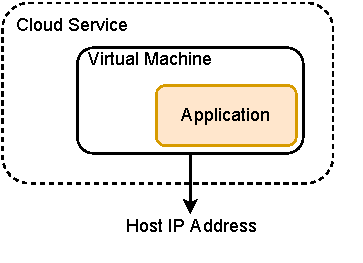
\includegraphics[width=0.45\linewidth]{images/Pattern-1.pdf}
        \caption{An example "application" is used for visualizing the pattern mentioned here.}
    \end{figure}  

In this pattern of deploying a microserivce application, multiple service instances or the entire application is provisioned on a single physical or virtual host in a cloud service. This is also often the easiest and most traditional pattern which can also work well with other architectures \citep{Chr19}. The application once deployed runs on a well known port, such as port 8080, which allows for HTTPS traffic to be directed towards the host, using the hosts IP address \citep{Chr19}. 

There can be various benefits and drawbacks for using this pattern.  Firstly, similar services can be deployed and are able to run more efficiently as the services share the same operating system and server resources  \textbf{reducing communication time between services as they no longer have to communicate over the internet.} Since all the services or a set of services are deployed on the same machines, they do not need to wait for other services in the application to start up, and can be easily deployed again or restarted. 

Whilst the benefits makes it an appealing pattern to use, there are also some drawback's, as multiple services run on the same host, there is minimal isolation between the services, making it harder to accurately track resource utilization per service, and a misbehaving services could consume a major chunk of the resource availability. 

\textit{Another known issue occurs since multiple services are to be deployed on the same server, each service needs to be documented well and have it's own configuration file for dependencies, if these are not well maintained, the complexity of figuring out which service is missing dependencies increase's complexity at the deployment stage.  }



\subsection{Pattern 2 : Multiple Service Instance per Multiple Hosts}
    \begin{figure}[H]
        \centering
        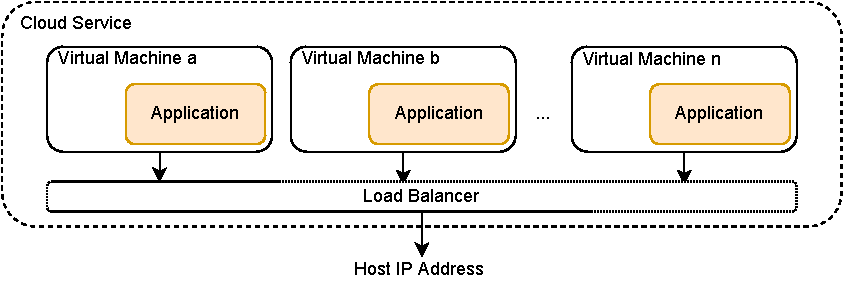
\includegraphics[width=0.9\linewidth]{images/Pattern-2.pdf}
        \caption{An example application is used for visualizing the pattern mentioned here.}
    \end{figure}  

This pattern is quite similar to Pattern 1, with the key difference being where multiple machine are provisioned to run multiple instances of the services.   


\subsection{Pattern 3 : Single service instance per multiple hosts}
    \begin{figure}[H]
        \centering
        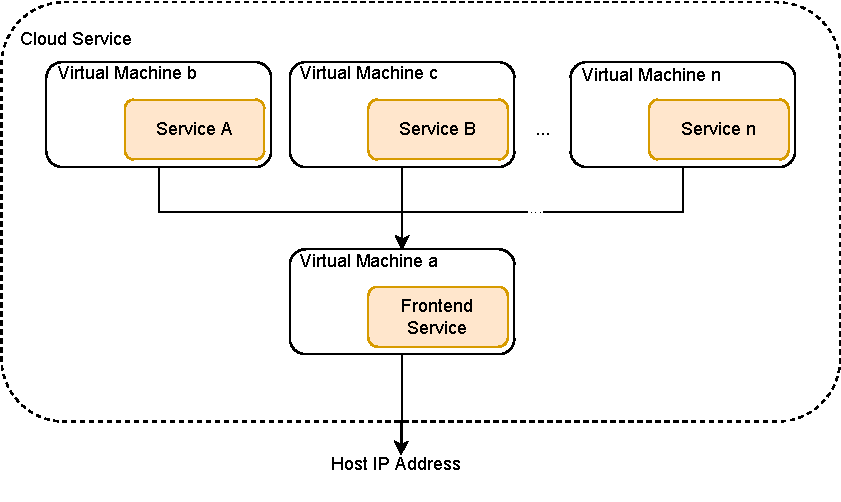
\includegraphics[width=0.8\linewidth]{images/Pattern-3.pdf}
        \caption{An example application is used for visualizing the pattern mentioned here.}
    \end{figure}  



\section{Infrastructure As A Platform -Terraform}
% https://amazicworld.com/building-auto-scaling-groupss-in-azure-with-terraform/

The Infrastructure as code platform used for the project is an open source tool developed by HashiCorp called Terraform, it uses a declarative language to deploy and manage infrastructure across a variety of cloud providers, private clouds and virtualization platforms. 


\subsection{Terraform Azure}
\begin{lstlisting}
    terraform {
      required_providers {
        azurerm = {
          source = "hashicorp/azurerm"
          version = "~>2.0"
        }
      }
    }
    
    # Use a pre-created resource group
    data "azurerm_resource_group" "{resource_name}" {
    	name = "{resource_name}"
    }
    
\end{lstlisting}

\subsection{Modules}
Modules are used to create light weight abstractions which can be used to describe infrastructure in terms of the architecture instead of fixed variable names. 
\subsubsection{Root Module}
\subsubsection{Child Modules}

%==================================================================================================================================

\chapter{Analysis and Requirements}\label{chp:AnR}
This chapter explores the different steps that have been taken to create the following architectures talked in chapter 4 Design, using the MoSCoW technique helped manage requirements throughout the project. Which is followed by a list of objects which have been identified for the dissertation. 
(ONE OF THIS MUST GO!)
\section{Requirements - MoSCoW}
\begin{itemize}
  \item Must
  \begin{itemize}
        \item There must be more than one application to deploy and test.
        \item There must be a load generator that simulates real-user usage. 
        \item There must be a workflow for deploying and testing applications
  \end{itemize}
  \item Should
  \begin{itemize}
    \item There should be at least 3 deployment patterns 
    \item There should be the ability to deploy the applications multiple times in one go. 
    \item There should be the ability to collect all possible metrics for both the machines and API.
  \end{itemize}
    \item Could
  \begin{itemize}
    \item There could be 
  \end{itemize}
\end{itemize}



\section{Research Objectives}
To create a suitable deployment and testing environment for the various patterns, the project is split into the following objectives:  
\begin{itemize}
    \item \textbf{O1} Identify suitable patterns for microservice deployments. 
    \item \textbf{O2} Identify open-source applications based on the microservice architecture to be used for testing patterns. 
    \item \textbf{O3} Create a modular and reproducible setup for deploying applications within different patterns. 
    \item \textbf{O4} Create a modular and reproducible setup for deploying load machines for the applications.
    \item \textbf{O5} Create a workflow for collecting and analysing machine and api metrics.
\end{itemize}
%==================================================================================================================================
\chapter{Design}\label{chap:design}

% This chapter takes inspiration from existing deployment patterns for microservices discussed in the previous chapter(BACKGROUND), which leads onto the creation of an architecture, comprising of multiple modules which are used to deploy, test and analyse different deployment patterns using a series of applications.  

% To create the final architecture, the application's deployment and testing have been split into two components allowing them be modular which increase's ease of use, which is then followed by the analysis component where collected data is converted to human readable information. 
% =======

% This chapter discusses the architecture required to create a suitable testing environment to deploy, test and analyse patterns on a cloud platform. 

% To create the final design for the architecture, it has been split into multiple components, where the components deploy, test and analyse the different patterns. 

% =========
This chapter discusses the design of the architecture required to create a suitable testing platform which builds up from the requirements discussed in the chapter \ref{chp:AnR}. The architecture is split into three different components, allowing it to deploy, test and analyse different patterns on a cloud platform. 

(Probs add a section above this which discusses why you need to deploy a pattern and that it requires different applications?)
\section{Components}
% % % % % % % % % % % % % % % % % % % % % % % % % % % % % % % % 

\begin{figure}[H]

\begin{minipage}{.5\linewidth}
\centering
\subfloat[Application Component]{\label{fig:application_comp}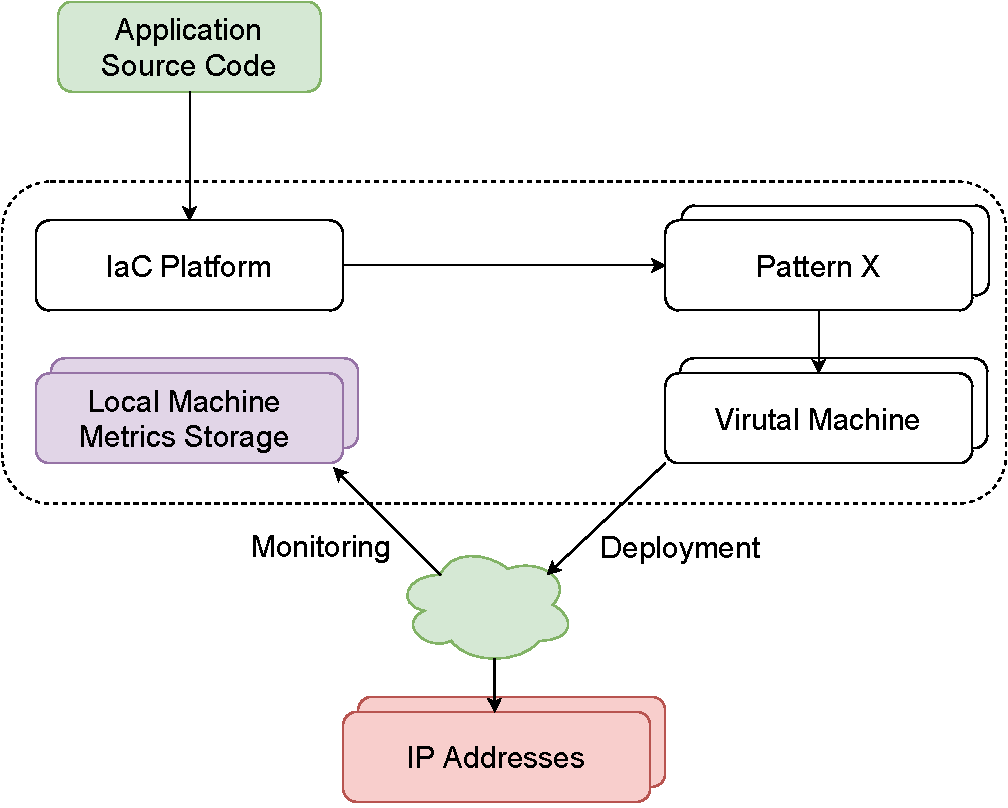
\includegraphics[scale=.36]{images/Modular_Application.pdf}}
\end{minipage}%
\begin{minipage}{.5\linewidth}
\centering
\subfloat[Testing Component]{\label{fig:testing_comp}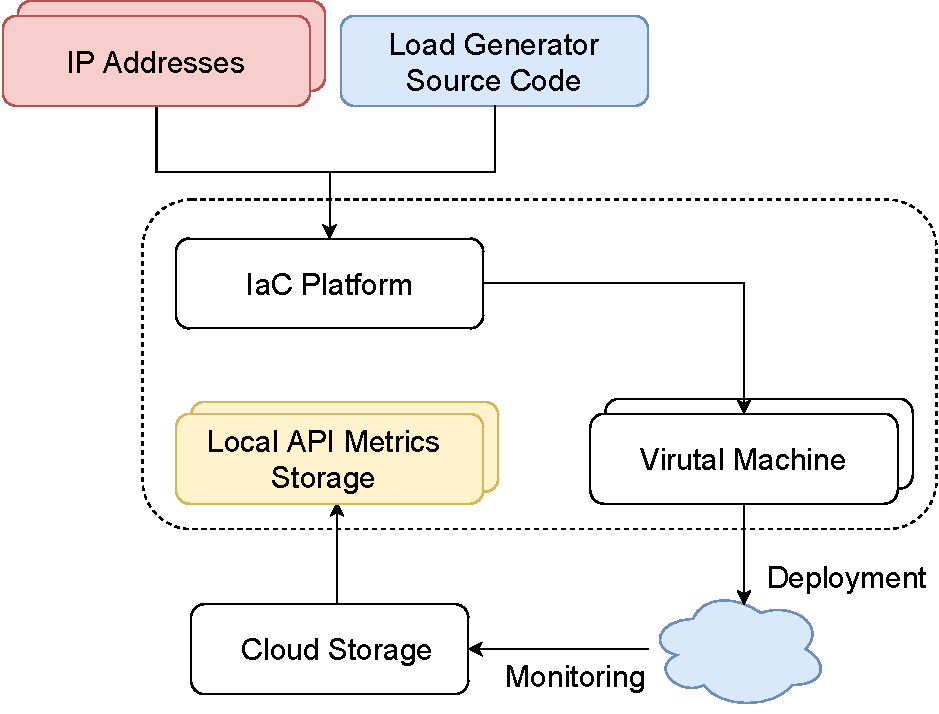
\includegraphics[scale=.4]{images/modular_load.pdf}}
\end{minipage}\par\medskip
\centering
\subfloat[Data Analysis Component]{\label{fig:analysis_comp}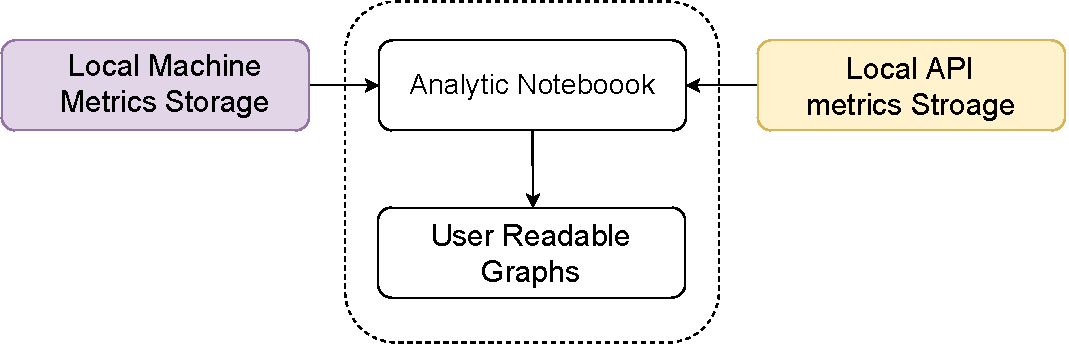
\includegraphics[scale=.4]{images/Data Flow.pdf}}
\caption{Three separate components which are used in the final architecture.}
\label{fig:main}
\end{figure}

% % % % % % % % % % % % % % % % % % % % % % % % % % % % % % % % 
\subsection{Application Component}
% \begin{figure}[H]
%     \centering
%     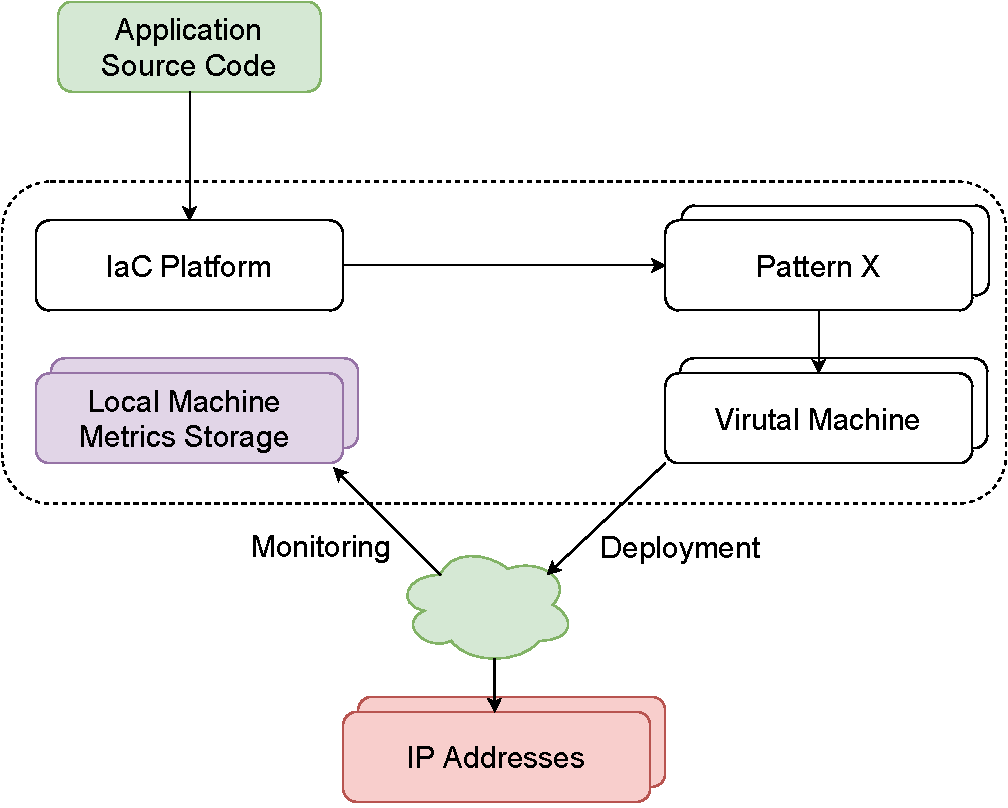
\includegraphics[width=0.7\linewidth]{images/Modular_Application.pdf}
%     \caption{Application component example using Pattern 1.}
%     \label{fig:application_comp}
% \end{figure} 

The component, as shown in sub-figure \ref{fig:application_comp}, accepts application source code, which is provisioned by the IaC platform to create multiple virtual machines within the chosen pattern to the cloud. Followed by an output of new host IP addresses, to be used by the testing component. 

A modular design of such allows for the IaC platform to create multiple machines at a time, which can be used for executing multiple tests, helping in reducing time. Once the applications have been deployed to the cloud, the module is set to an ideal state.

Followed by the creation of the testing component and after that component has been completed, this component collects the machine metrics from the cloud provider storing them locally, followed up by clearing up all instances of the component in the cloud. 
% % % % % % % % % % % % % % % % % % % % % % % % % % % % % % % % 
\subsection{Testing Component}
% \begin{figure}[H]
%     \centering
%     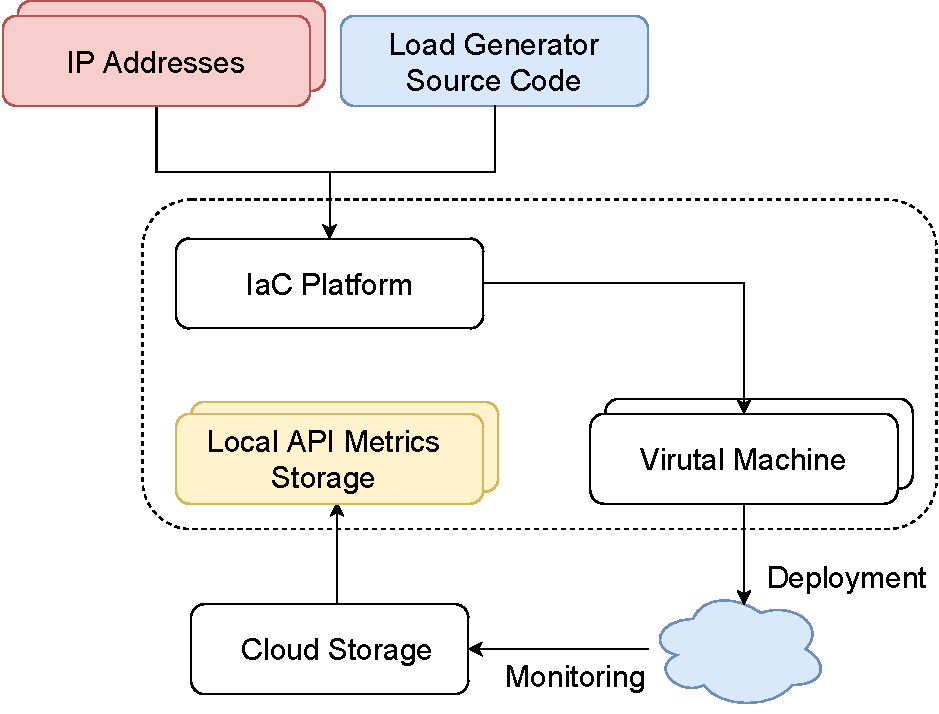
\includegraphics[width=0.7\linewidth]{images/modular_load.pdf}
%     \caption{Load Generator Component}
%     \label{fig:testing_comp}
% \end{figure} 
The component, as shown in figure \ref{fig:testing_comp}, the component accepts a list of host IP addresses generated by the application component, and the load generators source code. The list of IP addresses are now used by the IaC platform to create subsequent virtual machines which install the load generator and are then used to generate load for the deployed applications.

Once the load generator's have finished generating load, the output log file(s) are uploaded to the cloud storage, which are later downloaded locally. This is followed by clearing up all instances of the component in the cloud. 

% % % % % % % % % % % % % % % % % % % % % % % % % % % % % % % % 
\subsection{Analysis Component}

The analysis component shown in figure \ref{fig:analysis_comp}, reads in the machine's system metrics, such as memory usage and CPU usage, generated by the application component and load testings log files generated by the testing component, to create meaningful user readable information, this can be represented in a multitude of ways such as graphs or tables. 

\section{Final Architecture}
\begin{figure}[H]
    \centering
    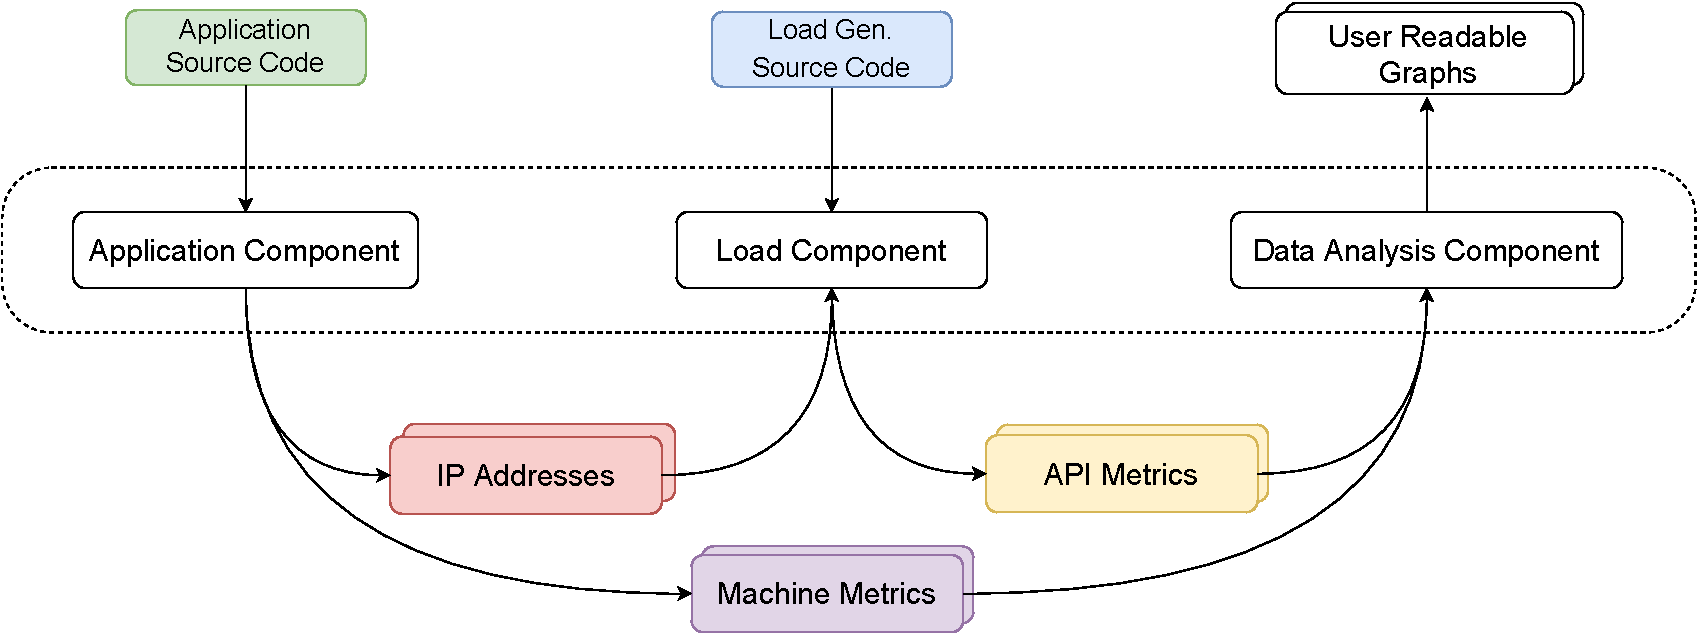
\includegraphics[width=1\linewidth]{images/final_arch.pdf}
    \caption{The final architecture, showing flow of information between each component.}
    \label{fig:final_arch}
\end{figure} 
The different components creates the final architecture as shown in figure 4.2, which outlays the various interactions between the components, the flow starts from the left side, ending to the right. (Should probs talk about how the integrations work, but unsure if that is needed) 

% The flow starts with a packaged microservice application, possibly stored on a version control system, where the source code for the application and load generator is kept separate from each other whilst also being easily accessible. 
% \\
% The source code follows two paths, controlled by the Main Script, where 
% \\
% \hspace*{6mm} \textbf{Path A} flows into the Infrastructure as a Code (IaC) platform which boots up a suitable virtual machine based on the requirements, such as deploying Pattern's one or two, which require modifications in the IaC script, once a machine is booted, the application can be hosted within the machine returning the Host's IP address with the application forwarded to the port address.
% \\
% \hspace*{6mm} \textbf{Path B} follows a similar path, however, skips out on the patterns, and is created after the application machine is hosted. Path A and B collide at this point, where B takes in the Host IP Address, and runs the load generator scripts for a certain amount of time, saving this data to the cloud provider so it can later be downloaded locally. 

% This is where the unit A's machine metrics are pulled from the provider and stored locally side by side to the API metrics. This concludes the use of both cloud machines and can be safely dropped. At the last stage of the workflow, both paths with the machine and API metrics flow into the analytical notebooks where data can be made sense of and compared to. 


%==================================================================================================================================

% 
\chapter{Implementation}
This chapter discusses the different technologies required to implement the architecture shown in figure \ref{fig:final_arch}, exploring why the technologies are an appropriate selection for the dissertation. 

\section{Applications}
To test different patterns, they require a selection of microservice based applications run under docker containers to deploy, the open-source community have built various microservice applications with different intents and features; for the purposes of testing patterns, three applications with different characteristics been chosen, allowing to simulate the different domains of microservices applications, such as a social media platform, or an e-commerce platform, making it possible to monitor effects it might have on different deployment patterns. This section further expands on the different applications and looks at their unique features and why these are a good contender for the analysis. 
\begin{figure}[H]
\begin{minipage}{.5\linewidth}
\centering
\subfloat[Social Network Architecture]{\label{fig:application_comp}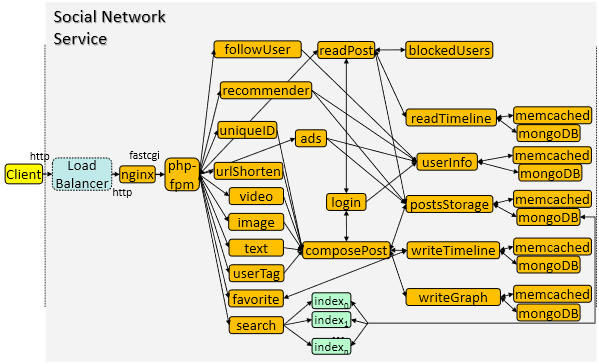
\includegraphics[scale=.4]{images/social_arch.png}}
\end{minipage}%
\begin{minipage}{.5\linewidth}
\centering
\subfloat[Hotel reservation Architecture]{\label{fig:testing_comp}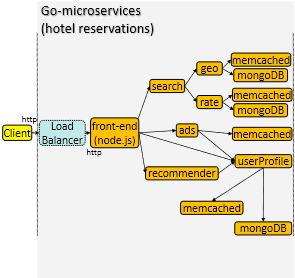
\includegraphics[scale=.53]{images/hotel_arch.png}}
\end{minipage}\par\medskip
\centering
\subfloat[Robot Shop Architecture]{\label{fig:analysis_comp}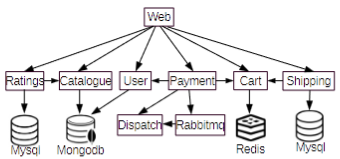
\includegraphics[scale=.65]{images/robot_shop_arch.png}}
\caption{This figure shows the different architectures for the chosen applications.}
\label{fig:application_architecures}
\end{figure}

% Talk about application features, such as number of microservice, what kinda things they look into. 
% referral links -> https://www.csl.cornell.edu/~delimitrou/papers/2019.asplos.microservices.pdf, https://www.instana.com/blog/stans-robot-shop-sample-microservice-application/, https://dl.acm.org/doi/pdf/10.1145/3297858.3304004

\textbf{Application 1: Stan’s Robot Shop}\\
\textbf{Scope:} This application is a simple e-commerce storefront based on customising and purchasing the robots and their parts. The application has been curated by developers at Instana and is to be used as a sandbox for learning orchestration and monitoring/observability techniques. \cite{Instana18}

\textbf{Functionality:} fig \ref{fig:robot_shop} shows the architecture of an end-to-end application, the front-end is a node.js server that talk's to the other services which are responsible for product catalogue, user repository, shopping cart, and order pipelines. \cite{Instana18}

\\
The following two applications are from an Open-source benchmark suite for cloud microservices, curated by the SAIL group at Cornell University. \cite{deathstar} 

\textbf{Application 2: Hotel Reservation}\\
\textbf{Scope:} This application is an online hotel reservation website, which is used for browsing information about hotels globally and making reservations, which uses the Go-microservice open-source project, and has been modified to add on backend databases, a machine learning widget used for advertisements and hotel recommendations. \cite{deathstar}

\textbf{Functionality:} fig \ref{fig:hotel_arch} shows the architecture of an end-to-end application, the front-end is a node.js server which talk's to the other services which are responsible for exploring hotel availability's in different regions and placing reservations, the back-end services use MongoDB storage for hotels and recommendations, with Memcached for caching. \cite{deathstar} 

\textbf{Application 3 : Social Network}\\
\textbf{Scope: }Social Network is an end-to-end microservice application, which implements a broadcast-style unidirectional relationships social network.  \cite{deathstar}

\textbf{Functionality:} fig \ref{fig:social_arch} shows the architecture of an end-to-end application, the front-end is a php-fqm service that talk's to the other services which are responsible for composing and displaying posts, and also the other services responsible for advertisements, search engines, etc. The messages are passed through using Apache Thrift RPC, the application also includes services for ads and recommender engines that use machine learning plugins hence. The back-end services use MongoDB storage for posts, media, profiles and recommendations, and Memcached for caching.   \cite{deathstar}


\begin{table}[H]
    
    \centering % used for centering table
    \begin{tabular}{c c c c} % centered columns (4 columns)
    \toprule\toprule %inserts double horizontal lines
     Service & Unique Microservices & Per-Language LoC Breakdown \\ [1ex] % inserts table
    %heading
    \toprule % inserts single horizontal line
    Stan's Robot Shop   & 7   & \begin{tabular}{@{}c@{}}30\% C, 21\% C++, 20\% Java, \\10\% PHP, 8\% Scala, 5\% node, 3\% Python, 3\% JS\end{tabular} \\ [2.5ex] 
    
    Hotel Reservation     & 15  & \begin{tabular}{@{}c@{}} 89\% Go, 7\% HTML, 4\% Python \end{tabular}  \\ [1.5ex]

    Social Network  & 36   &  \begin{tabular}{@{}c@{}}
    42.5\% JavaScript, 12.3\% PHP, 12.3\% Java, \\8.6\% HTML, 7.6\% Python, 7.4\% Shell
    \end{tabular}  \\ [0.5ex]

    \toprule %inserts single line
    \end{tabular}
    \caption{Characteristics and code composition of each microservices application} % title of Table\\

    \label{table:services} % is used to refer this table in the text
\end{table}


\section{Load Generators}
This section talks about the two different load generators which have been modified by the application developers to generate simulated load for the applications.

To evaluate the applications, and their behaviour behind 

(Explain why a loadd gen is needed) 



% https://dl.acm.org/doi/pdf/10.1145/3418688.3418691
% http://docs.locust.io/en/stable/what-is-locust.html#features

\textbf{Locust: }is an open-source easy use, scriptable and scalable performance testing tool. Allows for basic packet sending capabilities, and has been designed for performance testing websites and systems to test for concurrent user support. The tool runs completely on Python and allows the tester to write Locust test scripts entirely in python without adding complexity some other generators may generate load via a UI or XML files. 


\textbf{Wrk2 (Shuang's version): }




\section{Implementing Fruit Cocktail}
Fruit cocktail consists of multiple applications which are deployed with different patterns, as two patterns are to be tested, these require different directories to be created, in which these have two very similar structures however change with the terraform child modules. same structure which follows a combination of the Application Architecture and Load Architecture, as seen in the \autoref{chap:design}. 

(EXPLAIN THE TOP PARA BETTER)

The different architecture combinations, have been implemented using the various technologies described above. This section will breakdown each architectural module and talk about the various specifics in how it has been implemented before going over the integration between the two modules and analytical modules. 

\subsection{Deployment}

To deploy the architecture described in Figure \ref{fig:final_arch}, Terraform by Hashicorp and Azure by Microsoft have been used in combination.

% https://docs.microsoft.com/en-us/azure/developer/terraform/overview
% https://blog.gruntwork.io/why-we-use-terraform-and-not-chef-puppet-ansible-saltstack-or-cloudformation-7989dad2865c#.63ls7fpkq

Terraform, is an open-source tool, which allows to provision immutable cloud infrastructure (https://www.hashicorp.com/resources/what-is-mutable-vs-immutable-infrastructure),  achieved by writing template-based configuration files, which describe the topology of cloud resources; such as virtual machines, resource groups, load-balancers or storage accounts. (The Terraform CLI allows to deploy and version different templates to Azure.  )

% https://blog.gruntwork.io/how-to-create-reusable-infrastructure-with-terraform-modules-25526d65f73d
% https://learn.hashicorp.com/tutorials/terraform/module

A set of the configuration files in a single directory are known as a \textbf{module}. These have several advantages, such as splitting multiple configuration files into various logical components, allowing to re-use configuration files, providing consistency throughout and ensuring best practices. 

Terraform uses standard terminology to describe its modular functionalities; the leading working directory is known as the root module and uses \textit{module blocks} to call child modules, which could be loaded from the local file system or a remote source; Terraform Registry, Terraform Cloud, version control systems, etc.  

% Add code listing showing a sample module block / and loading a child module


which easily integrates with Azure, a cloud computing platform by Microsoft, which provides various services that allow to deployment cloud-based virtual machines in various configurations and regions. 


\textbf{Terraform} is used with-in the application and testing components, shown in Figures  \ref{fig:application_architecures}, \ref{fig:testing_comp} as this allows to deploy multiple instances of the application and load generators machines at once, Terraform also 


\subsection{Infrastructure as Cloud}



\subsection{Configuration Files}
These are two files stored under an \path{artifacts} directory, the first \path{machines.txt} allows for the code to identify a list of Azure machines sizes and the other \path{units.txt} is used to identify a list of units, these units often an alphanumeric word or letter are used to track and create multiple machines with their dependencies on Azure.

\subsection{Main Architecture}
Since Terraform is an infrastrcure as code platform and does not allow to pull metrics off the cloud or initialize multiple scrpits, a bash script has been used to..

\textbf{There are two ways in which the application component was implmenets, one for patten 1 and the other for pattern 2, can talk about this here and split application component into two sections. }
\subsection{Application Component}
With-in the architectures working directory a root module \path{main.tf} reads the \path{units.txt}, creating a list of units through local values, which allows repetitive use within the module. Next the root module uses an \path{application} block to call for a child module which is sourced locally from \path{/modules/services/application}, this child module stores the different resource blocks which describes the infrastructure objects collectively used by Azure to create the virtual machines in the cloud. 

The use of a child module with local values, allows for terraform to create 

\begin{lstlisting}[ float, caption={caption here}, label=lst:callahan]
  
locals {
 ips = split("\n", file("../artifacts/units.txt"))
}
...
module "application_a" {
  source = "../modules/services/application"

  for_each = toset( local.ips )
  unit_name = each.value
  ...
}

\end{lstlisting}

\subsection{Testing Component}

\subsection{Data Analytical Component}
Juypter notebooks take a part in this architecture as they allow to create reproducible notebooks for different tests, whilst keeping Independence from each test and making it easier to distinguish from each other. (?)

Once the files have been saved these are then organized in a new directory which can be read

% What did you do to implement this idea, and what technical achievements did you make?
% \section{Guidance}
% You can't talk about everything. Cover the high level first, then cover important, relevant or impressive details.



% \section{General points}

% These points apply to the whole dissertation, not just this chapter.



% \subsection{Figures}
% \emph{Always} refer to figures included, like Figure \ref{fig:relu}, in the body of the text. Include full, explanatory captions and make sure the figures look good on the page.
% You may include multiple figures in one float, as in Figure \ref{fig:synthetic}, using \texttt{subcaption}, which is enabled in the template.



% % Figures are important. Use them well.
% \begin{figure}
%     \centering
%     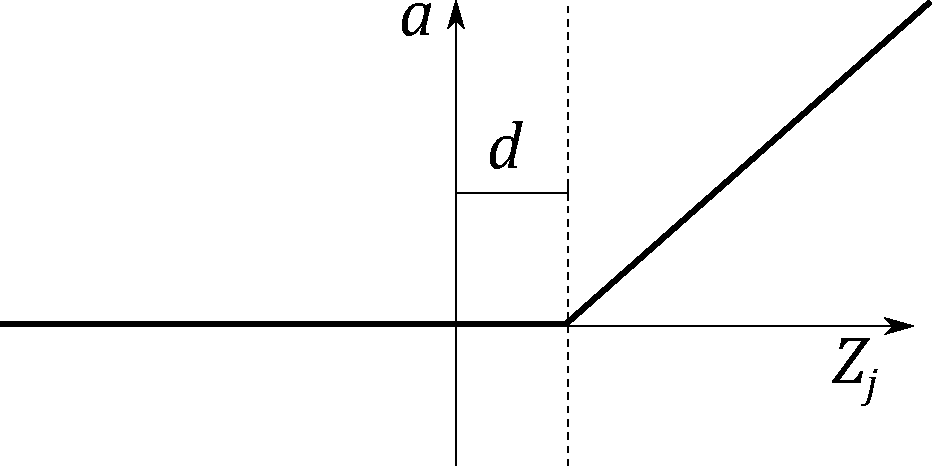
\includegraphics[width=0.5\linewidth]{images/relu.pdf}    

%     \caption{In figure captions, explain what the reader is looking at: ``A schematic of the rectifying linear unit, where $a$ is the output amplitude,
%     $d$ is a configurable dead-zone, and $Z_j$ is the input signal'', as well as why the reader is looking at this: 
%     ``It is notable that there is no activation \emph{at all} below 0, which explains our initial results.'' 
%     \textbf{Use vector image formats (.pdf) where possible}. Size figures appropriately, and do not make them over-large or too small to read.
%     }

%     % use the notation fig:name to cross reference a figure
%     \label{fig:relu} 
% \end{figure}


% \begin{figure}
%     \centering
%     \begin{subfigure}[b]{0.45\textwidth}
%         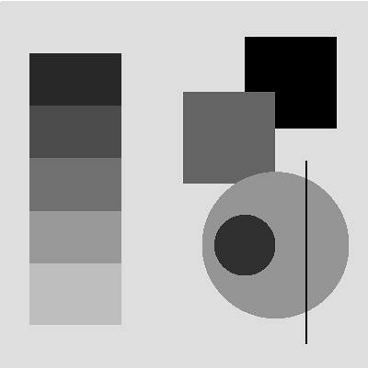
\includegraphics[width=\textwidth]{images/synthetic.png}
%         \caption{Synthetic image, black on white.}
%         \label{fig:syn1}
%     \end{subfigure}
%     ~ %add desired spacing between images, e. g. ~, \quad, \qquad, \hfill etc. 
%       %(or a blank line to force the subfigure onto a new line)
%     \begin{subfigure}[b]{0.45\textwidth}
%         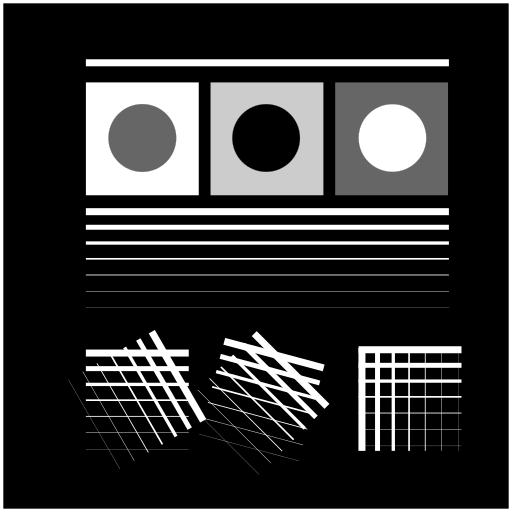
\includegraphics[width=\textwidth]{images/synthetic_2.png}
%         \caption{Synthetic image, white on black.}
%         \label{fig:syn2}
%     \end{subfigure}
%     ~ %add desired spacing between images, e. g. ~, \quad, \qquad, \hfill etc. 
%     %(or a blank line to force the subfigure onto a new line)    
%     \caption{Synthetic test images for edge detection algorithms. \subref{fig:syn1} shows various gray levels that require an adaptive algorithm. \subref{fig:syn2}
%     shows more challenging edge detection tests that have crossing lines. Fusing these into full segments typically requires algorithms like the Hough transform.
%     This is an example of using subfigures, with \texttt{subref}s in the caption.
%     }\label{fig:synthetic}
% \end{figure}

% \clearpage

% \subsection{Equations}

% Equations should be typeset correctly and precisely. Make sure you get parenthesis sizing correct, and punctuate equations correctly 
% (the comma is important and goes \textit{inside} the equation block). Explain any symbols used clearly if not defined earlier. 

% For example, we might define:
% \begin{equation}
%     \hat{f}(\xi) = \frac{1}{2}\left[ \int_{-\infty}^{\infty} f(x) e^{2\pi i x \xi} \right],
% \end{equation}    
% where $\hat{f}(\xi)$ is the Fourier transform of the time domain signal $f(x)$.

% \subsection{Algorithms}
% Algorithms can be set using \texttt{algorithm2e}, as in Algorithm \ref{alg:metropolis}.

% % NOTE: line ends are denoted by \; in algorithm2e
% \begin{algorithm}
%     \DontPrintSemicolon
%     \KwData{$f_X(x)$, a probability density function returing the density at $x$.\; $\sigma$ a standard deviation specifying the spread of the proposal distribution.\;
%     $x_0$, an initial starting condition.}
%     \KwResult{$s=[x_1, x_2, \dots, x_n]$, $n$ samples approximately drawn from a distribution with PDF $f_X(x)$.}
%     \Begin{
%         $s \longleftarrow []$\;
%         $p \longleftarrow f_X(x)$\;
%         $i \longleftarrow 0$\;
%         \While{$i < n$}
%         {
%             $x^\prime \longleftarrow \mathcal{N}(x, \sigma^2)$\;
%             $p^\prime \longleftarrow f_X(x^\prime)$\;
%             $a \longleftarrow \frac{p^\prime}{p}$\;
%             $r \longleftarrow U(0,1)$\;
%             \If{$r<a$}
%             {
%                 $x \longleftarrow x^\prime$\;
%                 $p \longleftarrow f_X(x)$\;
%                 $i \longleftarrow i+1$\;
%                 append $x$ to $s$\;
%             }
%         }
%     }
    
% \caption{The Metropolis-Hastings MCMC algorithm for drawing samples from arbitrary probability distributions, 
% specialised for normal proposal distributions $q(x^\prime|x) = \mathcal{N}(x, \sigma^2)$. The symmetry of the normal distribution means the acceptance rule takes the simplified form.}\label{alg:metropolis}
% \end{algorithm}

% \subsection{Tables}

% If you need to include tables, like Table \ref{tab:operators}, use a tool like https://www.tablesgenerator.com/ to generate the table as it is
% extremely tedious otherwise. 

% \begin{table}[]
%     \caption{The standard table of operators in Python, along with their functional equivalents from the \texttt{operator} package. Note that table
%     captions go above the table, not below. Do not add additional rules/lines to tables. }\label{tab:operators}
%     %\tt 
%     \rowcolors{2}{}{gray!3}
%     \begin{tabular}{@{}lll@{}}
%     %\toprule
%     \textbf{Operation}    & \textbf{Syntax}                & \textbf{Function}                            \\ %\midrule % optional rule for header
%     Addition              & \texttt{a + b}                          & \texttt{add(a, b)}                                    \\
%     Concatenation         & \texttt{seq1 + seq2}                    & \texttt{concat(seq1, seq2)}                           \\
%     Containment Test      & \texttt{obj in seq}                     & \texttt{contains(seq, obj)}                           \\
%     Division              & \texttt{a / b}                          & \texttt{div(a, b) }  \\
%     Division              & \texttt{a / b}                          & \texttt{truediv(a, b) } \\
%     Division              & \texttt{a // b}                         & \texttt{floordiv(a, b)}                               \\
%     Bitwise And           & \texttt{a \& b}                         & \texttt{and\_(a, b)}                                  \\
%     Bitwise Exclusive Or  & \texttt{a \textasciicircum b}           & \texttt{xor(a, b)}                                    \\
%     Bitwise Inversion     & \texttt{$\sim$a}                        & \texttt{invert(a)}                                    \\
%     Bitwise Or            & \texttt{a | b}                          & \texttt{or\_(a, b)}                                   \\
%     Exponentiation        & \texttt{a ** b}                         & \texttt{pow(a, b)}                                    \\
%     Identity              & \texttt{a is b}                         & \texttt{is\_(a, b)}                                   \\
%     Identity              & \texttt{a is not b}                     & \texttt{is\_not(a, b)}                                \\
%     Indexed Assignment    & \texttt{obj{[}k{]} = v}                 & \texttt{setitem(obj, k, v)}                           \\
%     Indexed Deletion      & \texttt{del obj{[}k{]}}                 & \texttt{delitem(obj, k)}                              \\
%     Indexing              & \texttt{obj{[}k{]}}                     & \texttt{getitem(obj, k)}                              \\
%     Left Shift            & \texttt{a \textless{}\textless b}       & \texttt{lshift(a, b)}                                 \\
%     Modulo                & \texttt{a \% b}                         & \texttt{mod(a, b)}                                    \\
%     Multiplication        & \texttt{a * b}                          & \texttt{mul(a, b)}                                    \\
%     Negation (Arithmetic) & \texttt{- a}                            & \texttt{neg(a)}                                       \\
%     Negation (Logical)    & \texttt{not a}                          & \texttt{not\_(a)}                                     \\
%     Positive              & \texttt{+ a}                            & \texttt{pos(a)}                                       \\
%     Right Shift           & \texttt{a \textgreater{}\textgreater b} & \texttt{rshift(a, b)}                                 \\
%     Sequence Repetition   & \texttt{seq * i}                        & \texttt{repeat(seq, i)}                               \\
%     Slice Assignment      & \texttt{seq{[}i:j{]} = values}          & \texttt{setitem(seq, slice(i, j), values)}            \\
%     Slice Deletion        & \texttt{del seq{[}i:j{]}}               & \texttt{delitem(seq, slice(i, j))}                    \\
%     Slicing               & \texttt{seq{[}i:j{]}}                   & \texttt{getitem(seq, slice(i, j))}                    \\
%     String Formatting     & \texttt{s \% obj}                       & \texttt{mod(s, obj)}                                  \\
%     Subtraction           & \texttt{a - b}                          & \texttt{sub(a, b)}                                    \\
%     Truth Test            & \texttt{obj}                            & \texttt{truth(obj)}                                   \\
%     Ordering              & \texttt{a \textless b}                  & \texttt{lt(a, b)}                                     \\
%     Ordering              & \texttt{a \textless{}= b}               & \texttt{le(a, b)}                                     \\
%     % \bottomrule
%     \end{tabular}
%     \end{table}
% \subsection{Code}

% Avoid putting large blocks of code in the report (more than a page in one block, for example). Use syntax highlighting if possible, as in Listing \ref{lst:callahan}.

% \begin{lstlisting}[language=python, float, caption={The algorithm for packing the $3\times 3$ outer-totalistic binary CA successor rule into a 
%     $16\times 16\times 16\times 16$ 4 bit lookup table, running an equivalent, notionally 16-state $2\times 2$ CA.}, label=lst:callahan]
%     def create_callahan_table(rule="b3s23"):
%         """Generate the lookup table for the cells."""        
%         s_table = np.zeros((16, 16, 16, 16), dtype=np.uint8)
%         birth, survive = parse_rule(rule)

%         # generate all 16 bit strings
%         for iv in range(65536):
%             bv = [(iv >> z) & 1 for z in range(16)]
%             a, b, c, d, e, f, g, h, i, j, k, l, m, n, o, p = bv

%             # compute next state of the inner 2x2
%             nw = apply_rule(f, a, b, c, e, g, i, j, k)
%             ne = apply_rule(g, b, c, d, f, h, j, k, l)
%             sw = apply_rule(j, e, f, g, i, k, m, n, o)
%             se = apply_rule(k, f, g, h, j, l, n, o, p)

%             # compute the index of this 4x4
%             nw_code = a | (b << 1) | (e << 2) | (f << 3)
%             ne_code = c | (d << 1) | (g << 2) | (h << 3)
%             sw_code = i | (j << 1) | (m << 2) | (n << 3)
%             se_code = k | (l << 1) | (o << 2) | (p << 3)

%             # compute the state for the 2x2
%             next_code = nw | (ne << 1) | (sw << 2) | (se << 3)

%             # get the 4x4 index, and write into the table
%             s_table[nw_code, ne_code, sw_code, se_code] = next_code

%         return s_table

% \end{lstlisting}

%==================================================================================================================================
\chapter{Evaluation} 
How good is your solution? How well did you solve the general problem, and what evidence do you have to support that?

\section{Guidance}
\begin{itemize}
    \item
        Ask specific questions that address the general problem.
    \item
        Answer them with precise evidence (graphs, numbers, statistical
        analysis, qualitative analysis).
    \item
        Be fair and be scientific.
    \item
        The key thing is to show that you know how to evaluate your work, not
        that your work is the most amazing product ever.
\end{itemize}

\section{Evidence}
Make sure you present your evidence well. Use appropriate visualisations, reporting techniques and statistical analysis, as appropriate.

If you visualise, follow the basic rules, as illustrated in Figure \ref{fig:boxplot}:
\begin{itemize}
\item Label everything correctly (axis, title, units).
\item Caption thoroughly.
\item Reference in text.
\item \textbf{Include appropriate display of uncertainty (e.g. error bars, Box plot)}
\item Minimize clutter.
\end{itemize}

See the file \texttt{guide\_to\_visualising.pdf} for further information and guidance.

\begin{figure}
    \centering
    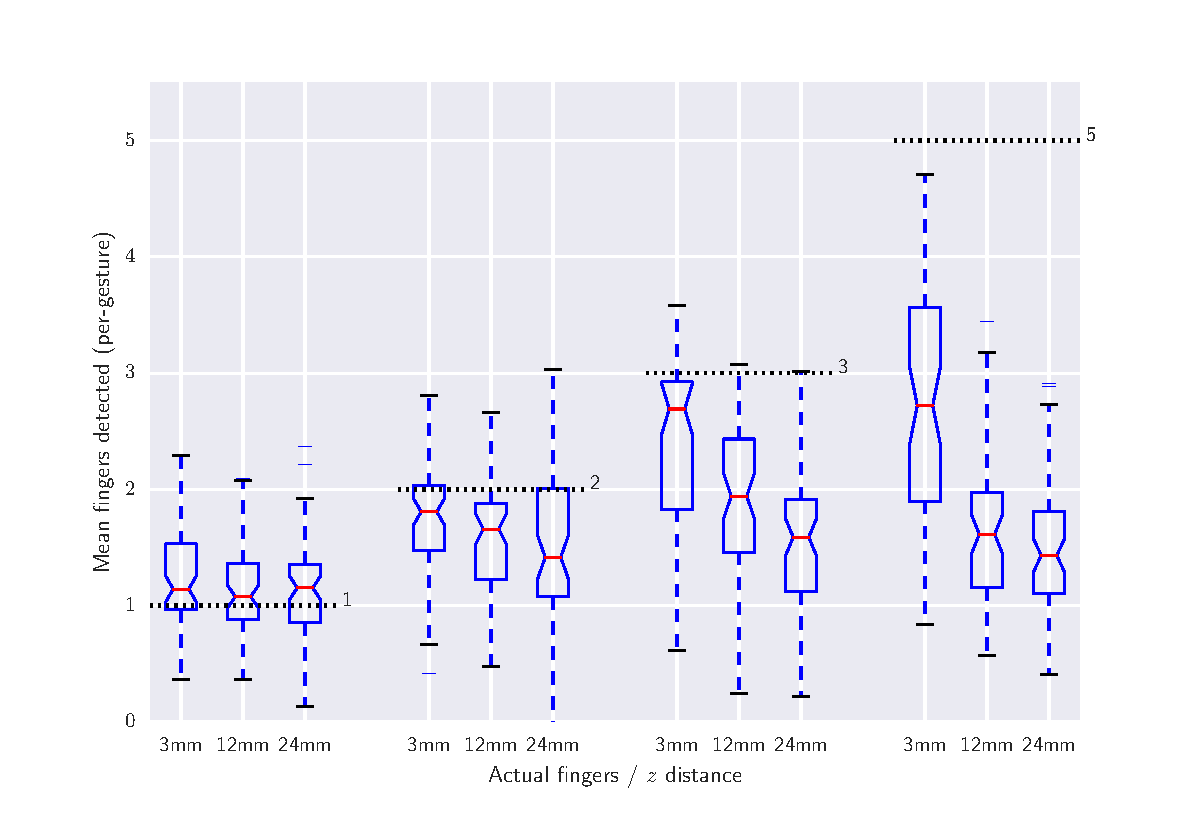
\includegraphics[width=1.0\linewidth]{images/boxplot_finger_distance.pdf}    

    \caption{Average number of fingers detected by the touch sensor at different heights above the surface, averaged over all gestures. Dashed lines indicate
    the true number of fingers present. The Box plots include bootstrapped uncertainty notches for the median. It is clear that the device is biased toward 
    undercounting fingers, particularly at higher $z$ distances.
    }

    % use the notation fig:name to cross reference a figure
    \label{fig:boxplot} 
\end{figure}
%==================================================================================================================================
\chapter{Conclusion}    
Summarise the whole project for a lazy reader who didn't read the rest (e.g. a prize-awarding committee).
\section{Future Works}

- There would be so much future work with this 
- Deploy and Test Pattern 3 with the machines
- Deploy the machines on different cloud types which are provided 
- Use a standardized workload generator for each. 


\section{Summary}
\begin{itemize}
    \item
        Summarise briefly and fairly.
    \item
        You should be addressing the general problem you introduced in the
        Introduction.        
    \item
        Include summary of concrete results (``the new compiler ran 2x
        faster'')
    \item
        Indicate what future work could be done, but remember: \textbf{you
        won't get credit for things you haven't done}.
\end{itemize}
%==================================================================================================================================
%  APPENDICES  
\begin{appendices}

\chapter{Appendices}

Typical inclusions in the appendices are:

\begin{itemize}
\item
  Copies of ethics approvals (required if obtained)
\item
  Copies of questionnaires etc. used to gather data from subjects.
\item
  Extensive tables or figures that are too bulky to fit in the main body of
  the report, particularly ones that are repetitive and summarised in the body.

\item Outline of the source code (e.g. directory structure), or other architecture documentation like class diagrams.

\item User manuals, and any guides to starting/running the software.

\end{itemize}

\textbf{Don't include your source code in the appendices}. It will be
submitted separately.

\end{appendices}



\definecolor{foldercolor}{RGB}{124,166,198}

\forestset{is file/.style={edge path'/.expanded={%
        ([xshift=\forestregister{folder indent}]!u.parent anchor) |- (.child anchor)},
        inner sep=1pt},
    this folder size/.style={edge path'/.expanded={%
        ([xshift=\forestregister{folder indent}]!u.parent anchor) |- (.child anchor) pic[solid]{folder=#1}}, inner ysep=0.6*#1},
    folder tree indent/.style={before computing xy={l=#1}},
    folder icons/.style={folder, this folder size=#1, folder tree indent=4*#1},
    folder icons/.default={12pt},
}

% Move to appendix
\begin{forest}
    for tree={font=\sffamily, grow'=0,
    folder indent=.9em, folder icons,
    edge=densely dotted}
    [
      [artifacts
          [units.pdf, is file]
          [machines.pdf, is file]]
      [modules
          [
              [services
                [
                    application
                ]
                [
                    load
                ]
              ]
          ]
      ]
      [staging
        [
        ]
      ]
      [testing
        [
        ]
      ]
      [main.sh]
    ]
\end{forest}
%==================================================================================================================================
%   BIBLIOGRAPHY   

% The bibliography style is abbrvnat
% The bibliography always appears last, after the appendices.

\bibliographystyle{abbrvnat}

\bibliography{l4proj}

\end{document}
